\subsection{Soving the inverse kinematics of Lynxmotion by neural network (Mang Ning)}
\subsubsection{Neural network and back porpagation}
In essense, artificial neural network is a computational model that can approximate any functions. The structure of a network is formed by connecting each neuron through linear equation and specific activation function,which is expressed in equation (\ref{eq:nn_linear_equation}). Basically, the meaning of training a neural network is actually adjusting the variables $w$ and $b$ insides the linear function.  

\begin{equation}
\label{eq:nn_linear_equation}
a = \sigma(w_1a_1+w_2a_2+w_3a_3+...+w_na_n-b)
\end{equation}

Afterwards, our target is to minimize a cost function that measures the performance of the network . This function involves all variavles $w_i$ and $b_i$ which enable us to find the minimum value by computing the partial derivative   in terms of each $w_i$ and $b_i$. Then the cost function can be minimized along the partial derivative path just as shown in figure \ref{fig:gradient_descent}.

\begin{figure}[htbp] 
\begin{center}
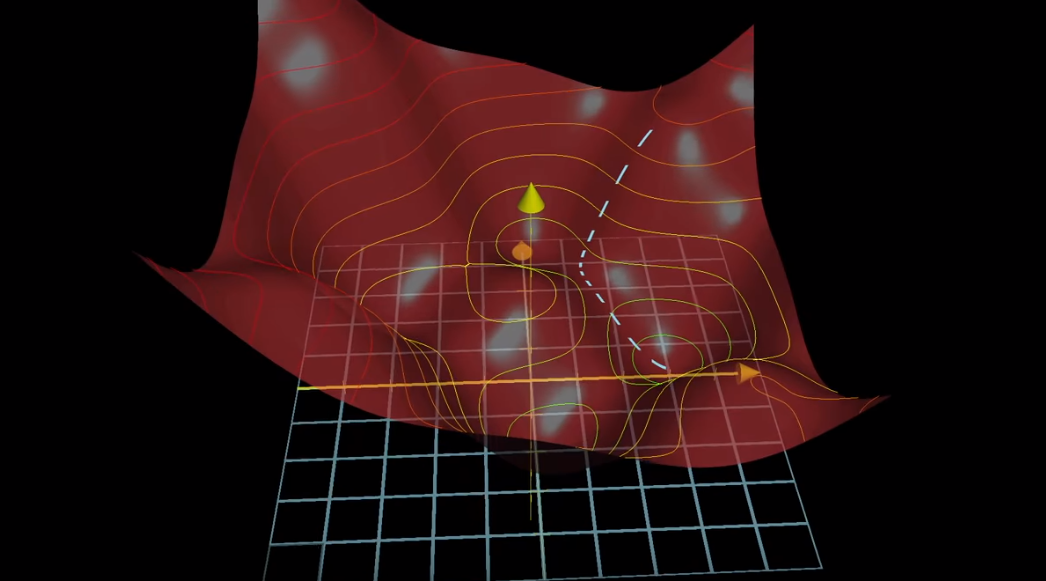
\includegraphics[width=\textwidth]{images/gradient_descent}
\caption{the process of reaching the minimum point of cost function by gradient descent}
\label{fig:gradient_descent}
\end{center}
\end{figure}

Next, back propagation algorithm can derive a specific variation for every $w_i$ and $b_i$ in each iteration. As a result, the training of a neural network will be completed and it can be used to make predictions.  

\subsubsection{Applying neural network on inverse Kinematics}
As for the structure of this neural network applied on inverse kinematics,the input should be 12 neurons since the rotation and translation have 12 elements totally. Similarly, the output layer has 5 neurons for $\theta_1...\theta_5$(ignoring the redundant sulotion). Experientially, the number of hidden layers should be comparitive to the number of neurons of input layer. Thus, the structure can be expressed as figure \ref{fig:IK_neural_network}. 

\begin{figure}[htbp] 
\begin{center}
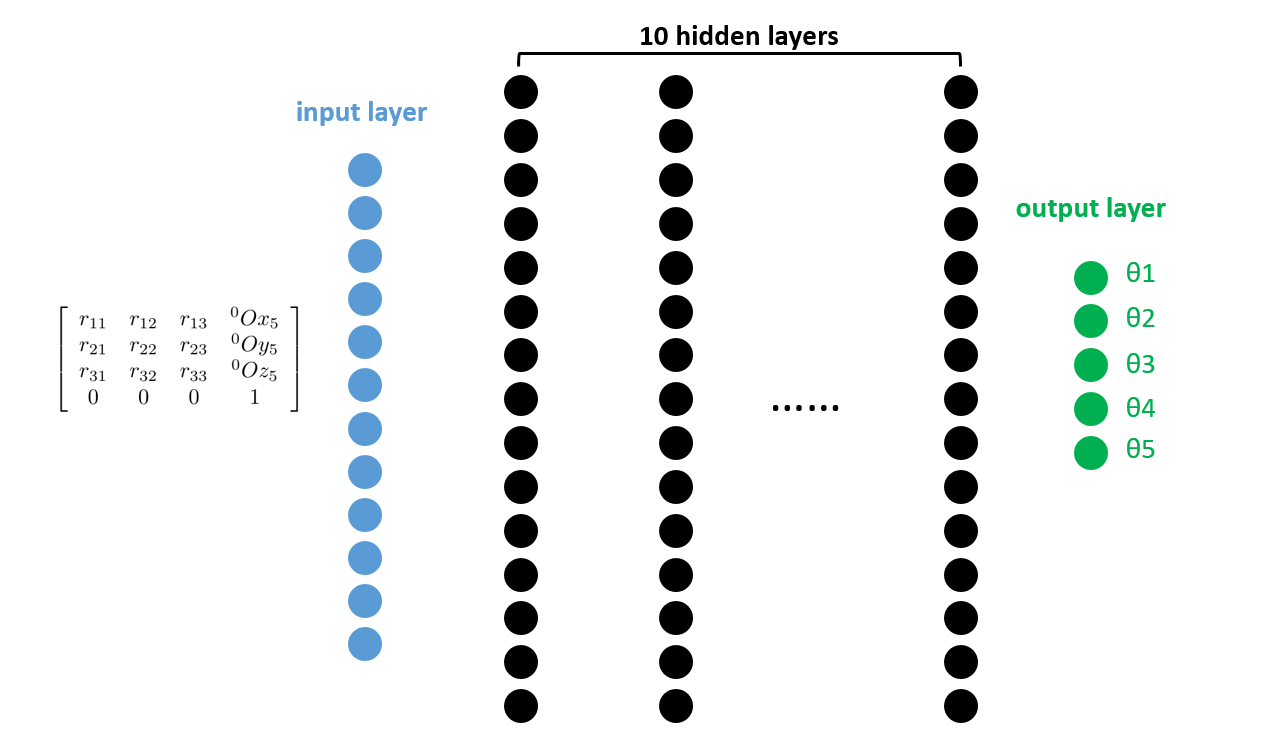
\includegraphics[width=\textwidth]{images/IK_neural_network}
\caption{the structure of the neural network applied in inverse kinematics}
\label{fig:IK_neural_network}
\end{center}
\end{figure}

A massive training data can be generated by previous forward kinematics code, concretely, $10^5$ data is created based on picking $10$ values uniformly for $\theta_1...\theta_5$ respectively. These data will be split into traning data and test data at a ratio of $0.8$.
After setting relevant learning parameters, the training of neural network can be excuted. For simplicity, we only adopt $\theta_3$ as the output because the training time will exceed hundreds hours if the network output $\theta_1$ to $\theta_5$ simultaneously. Besides, the range of joints angle is also contrained between $[0^{\circ},20^{\circ}$. 
It turns out that 





\subsubsection{Conclusion and future study}
network complexity, training time, accuracy, data volume 

momentum algorithm

continue here